% Author: Tony Lu Zhehao (tony1023@foxmail.com)
% 2AP2, International Cirriculum Center, Shenzhen Foreign Languages School, Shenzhen, China
% Date: July 30, 2016
% Done in Palo Alto
% Final paper for Pioneer Research Program 2015-2016 Spring (Physics: Investigating Gravitational Waves With LIGO Data)
% Instructor: Eric Myers

\documentclass[aps,prd,preprint]{revtex4}
%\documentclass[aps,prd,twocolumn,twoside,floatfix]{revtex4}

\usepackage{pioneer}
\def\theYear{2016}
\usepackage{graphicx}
\usepackage{bibentry}
\usepackage{csquotes}
\usepackage{listings}
\usepackage{courier}
\usepackage{subfig}

\begin{document}
\pagestyle{pioneer}
\date{July 30, 2016}
\preprint{}
\title{The Possibility of Earlier LIGO to Detect GW150914}
\author{Zhehao Lu}

\begin{abstract}
I report the results of my investigation on the sensitivity of LIGO at earlier stages. I took the waveform signal of the event GW150914 to make injections into the data from LIGO's S6 run and recovered the injections. Overall, none of signal-to-noise ratio values recovered was high enough to claim a detection. In the later portion of S6 where the noise was weaker, the signal could be identified as a candidate event at best. I compared the S6 run with the data from the earlier stages of LIGO and found that the equipment in earlier runs was insufficient to make the detection as well.
\end{abstract}
\maketitle



\section{The Main Questions}
One of the deciding factors that made the detection of elusive gravitational waves possible is the sensitivity of the equipment. Over LIGO's S5 \cite{S5}, S6 \cite{S6} and O1 \cite{Observation1} (which the scientists previously referred to as S7) runs, the sensitivity was improved significantly each time, with effective attenuation of noise (see section \ref{sec:compare}).
\par To some degree, the detection seemed very coincidential, for no detection in the past two decades was made until the one made just one week after the testing launch of Advanced LIGO \cite{timeline}. This leads to some questions: Was LIGO at any early stage sensitive enough to make this detection? Was the detection of GW150914 a coincidence?
%============================================================


\section{Background Information}
More than a century ago Albert Einstein's General Theory of Relativity stated that we live in a four-dimensional world\textemdash space-time (three dimensions for space and one for time). Mass causes distortions in space-time, which accounts for the phenomenon of gravity. The theory predicts that changing mass distribution will generally produce ripples in space-time, which is one of Einstein's predictions\textemdash gravitational waves \cite{relativity1,relativity2}. For decades, scientists have been struggling to detect gravitational waves from outer space. They upgraded their detectors over and over again, in order to catch the whispers of distant celestial bodies. Fortunately, on September 14, 2015, the LIGO detectors successfully recorded the signals from two colliding black holes, which was the first direct detection of gravitational waves ever, a remarkable one \cite{O1}. It was labeled GW150914.
\par This section aims to provide background information about LIGO and gravitational waves.
%---------------------------------------------------------------------------------------

\subsection{Introduction to Gravitational Waves \label{sec:GW}}
Einstein found that his linearized weak-field equations have wave solutions. \cite{O1} These transverse waves are \emph{ripples} in the \emph{fabric} of space-time, caused by some considerable and catastrophic events in the universe.
\par According to Einstein's calculations, gravitational waves are generated by objects accelerating with asymmetric motion. To be more precise, gravitational waves require changing quadrupole mass distribution. Generally, the amount of gravitational waves given off is positively correlated with the system's mass and its speed of motion. Changes in space-time produced by a moving mass are not felt in the distance immediately, but they propagate at the speed of light \cite{SBackground}.
\par Gravitational waves are transverse waves, the same as electromagnetic waves, but they are waves of changes in tensors (quadrupole distortions of space-time) which result in expansions and contractions of lengths in certain directions. Unlike the horizontal and vertical polarizations of electromagnetic waves, those of gravitational waves are \enquote{plus} and \enquote{cross}. However, gravitational waves do share lots of similarities with electromagnetic waves. They have frequencies and wavelengths, whose relationship is given by: $\lambda f=c$, where $\lambda$ is the wavelength, $f$ is the frequency, and $c$ is the speed of light. They are able to carry energy, momentum, and angular momentum away from the source \cite{SBackground}. The strain amplitude can be derived from Einstein's quadrupole formula, and it is inversely proportional to the distance from the mass center \cite{relativity1,relativity2}. It can also be measured by ratio of the change in length to the original length $h = \Delta L/L$. 
\begin{figure}
	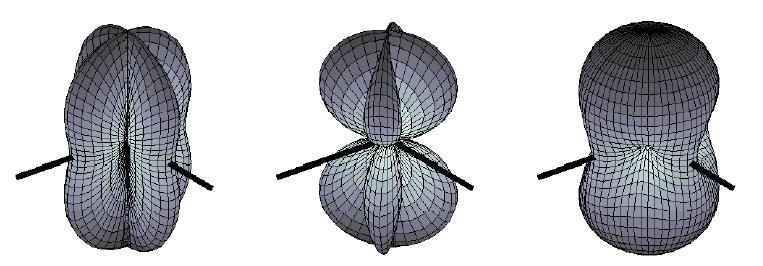
\includegraphics{G-wave_polarizations}
	\caption{The pattern on the left is for plus polarization, the middle pattern is for cross polarization, and the right one is for unpolarized waves. The black lines are the arms of LIGO detectors, which will be addressed in \ref{sec:LIGO}. \cite{instrument}}
\end{figure}
\par Gravitational waves have various sources, but there are mainly four categories: stochastic background, bursts from gravitational collapse, pulsars, and binary systems. Binary systems refer to those that consist of two bodies rotating around each other. Whether or not the two stars collide, gravitational waves will be generated. The detection made on September 14, 2015 is the collision of two black holes, which is called compact binary coalescence\textemdash \enquote{chirp}. \cite{O1} More details are given by a paper on gravitational waves in section three, in which the author addresses their sources \cite{SBackground}.
%---------------------------------------------------------------------------------------

\subsection{Introduction to LIGO \label{sec:LIGO}}
Distortions in space-time are almost impossible to measure directly, for if you use a meter stick, the meter stick, itself, will expand and contract with changing space-time. Fortunately, the speed of light remains the same despite any deformation of space-time, which sets the basis for the LIGO detectors \cite{CaltechLIGO}.
\par The detector of LIGO\textemdash Michelson Interferometer\textemdash was invented by Albert Abraham Michelson. The Micelson Interferometers were first applied in the famous Michelson-Morley experiment \cite{Michelson-Morley}. Its function is for optical interferometry. With a beam splitter, a light source is split into two arms, and each of the new beams is reflected back and combined again. The result of such combination leads to optical interference\textemdash either constructive or destructive\textendash depending on the changes in the length of the arms. Therefore, the photo detector could sense the variation in the arm lengths \cite{CaltechLIGO}.
\par The interferometer in LIGO consists of two vacuum arms of equal length\textemdash 4 kilometers long, forming an L shape. There is a laser light source and a photodetector at the corner of the L, as well as a beam splitter. At each end and in the middle of the arms are four freely-hanging mirrors which reflect the laser beam, and the two beams are combined into one at the beam splitter. Those mirrors in the middle are used to increase the distance that light beams travel, and as a result, the actual effective length is increased from 4km to 1120 km, greatly enhancing LIGO's sensitivity. If the arm lengths were to change, the two light beams that were originally in phase would be out of phase, creating destructive interference, which allows the photodetector to sense the infinitesimal change in the length of the arms \cite{CaltechLIGO, MitLIGO}.
\begin{figure}
	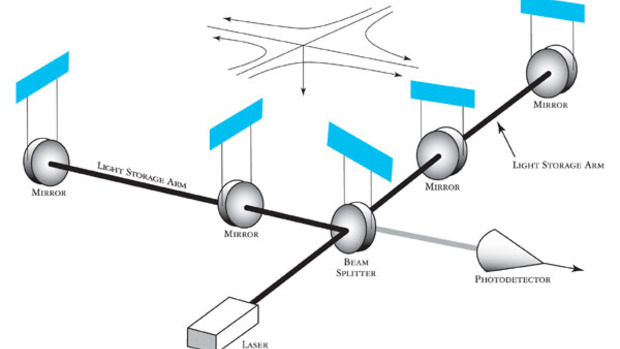
\includegraphics[scale = 0.7]{basic_ifo_diagram}
	\caption{Basic schematic of LIGO's interferometers with an incoming gravitational wave depicted as arriving from directly above the detector. \cite{CaltechLIGO}}
\end{figure}
\par The two LIGOs in the US are located in Livingston Parish, Louisiana and Hanford, Washington. Both are L-shaped and of the same size\textemdash their arms are all 4km long. The two Ls are in different directions, and they are separated by 3002 kilometers, which means the planes that these observatories are on form a nonzero dihedral angle \cite{DualDetector}. Therefore, it is guaranteed that gravitational waves from any direction can be detected, given enough sensitivity.
\par A brief history of LIGO is given on a Caltech's website \cite{BHLIGO}. A more technically and quantitatively detailed description of LIGO is given by the paper on LIGO's instruments \cite{instrument}.
%---------------------------------------------------------------------------------------

\subsection{Sensitivity of the Detectors}
Similar to any real physics experiment, the LIGO detectors face various disturbances from the environment. Considering the small amplitudes of gravitational waves, we see that sensitivity becomes decisive. At the very beginning of the construction, the interference of the noises was so high that it was impossible for the detectors to collect data clean enough to analyze. But the quality of data collected has been significantly improved over the several stages of LIGO. The datasets of its S5 (2005-2007) \cite{S5}, S6 (2009-2010) \cite{S6}, and O1 (September 2015-January 2016) \cite{Observation1} are available online \cite{TLdata}. Among all these sensitivity-limiting factors are primarily: seismic noise (at relatively low frequencies), thermal noise (at mid frequencies), shot noise (at high frequencies), and the problems with the lasers and electronics. Some more specific details, including solutions, are given by \cite{Noise, thermal, seismic}
\par The problems related to sensitivity are curious to investigate. My research is closely related to sensitivity.
%---------------------------------------------------------------------------------------

\subsection{Injections}
In short, injections were used to test whether the detectors were working well. There are two types of injections: hardware injections and software injections. The first type is made by manually changing the position of the mirrors in the interferometer. The second type is achieved by adding a signal directly into the data flow. Moreover, there were those called \enquote{blind injections}, when few scientists knew it was an injection while the majority were convinced that it was a real detection. One of the most famous events was in 2010, which was reported on the LSC news site \cite{blindInj}.
%=========================================================


\section{Preparation of Data Files \label{sec:dataFile}}
The strain data of the GW150914 event was be obtained from the LOSC site. Specifically, it was stored as a \enquote{\texttt{waveform.txt}} file from the \enquote{Download the Data} section in the LOSC tutorial \cite{GWTutorial}. This strain data was later used as the signal for the software injection.
\par As for the template for injection recovery, it is different from the waveform. It is included in the zip file of another tutorial \cite{GWTutorial2}. The complex template contains two waveforms, one of which is used as the real part and the other as the imaginary part, just like the configuration of a complex number. Moreover, as pointed out in the \enquote{Waveform Template} of this tutorial, the templates are not 100\% identical to what the scientists actually used. Many subtleties are skipped, for example. But the quality of the templates online is good enough for my investigation. Note that this is different from the strain data for making the injection.
\par The background strain data of the injections were selected from a number of datafiles in the \enquote{H1} detector from LIGO's S6 run, from GPS time 931035615 to 971622015 \cite{TimeConvert1,TimeConvert2}. The S6 data archive is available on the LOSC site as well \cite{S6Data}. Because of the probable fluctuation in the power of the background noise over the entire S6 run, 10 different and relatively evenly dispersed datafiles were chosen, each starting at GPS time 931127296 (0.226\%), 934846464 (9.39\%), 941707264 (26.3\%), 941785088 (26.5\%), 947154944 (39.7\%), 952623104 (53.2\%), 959344640 (69.8\%), 963629056 (80.3\%), 967442432 (89.7\%), and 971407360 (99.5\%), all lasting for 4096 seconds. The files will be referred to with numbers from 1 to 10, respectively.
\par The quality of background noise is critical. A piece of low-quality data could result in a misleading outcome. Furthermore, that kind of datafiles would be vetoed by the scientists. As a result, even if there really were an event, the segment it lies in would not be searched. And it would be useless to investigate such a datafile. In general, the background should have the proper data quality flags on. Because the event of GW150914 is a compact binary coalescence system \cite{O1} and the mass is big enough to be categorized as \enquote{high mass} \cite{S6himass}, the flag of \enquote{CBCHIGH\textunderscore CAT4} should be on. Besides, there should not be any other injections which would affect my recovery, so the flag of \enquote{HW} should be off. \cite{S6DQ} The specific way to slice qualified data segments is given in the code in appendix section \ref{sec:Appendix}.
\par The process of gathering the raw data for analysis could be categorized into two steps\textemdash making and recovering the software injection. The injections were made by simply superposing the waveform onto the background signal. Five injections were made into each of the ten datafiles at randomly selected points. In addition to the original strain, the waveform signal was amplified by factors ranging from 2 to 30, with a serial interval of 2, and was injected at the same points as those for the unamplified signal. In total, 800 injections were made. To recover the injection, signal-to-noise ratio (SNR) \cite{SNR} of each injection was computed with matched filter \cite{findChirp}. In addition, another set of recoveries were done with no injections in the datafile, which served as a check of the false alarms, the details of which will be addressed in section \ref{sec:SNR}. That was 850 SNR values in total. The signal processing was almost entirely the same as that in the tutorial on LOSC site \cite{GWTutorial}. The exact python code is given in the appendix section \ref{sec:Appendix} with more detailed description.
%=====================================================


\section{Data Analysis}
This section presents the data analyzing process.

\subsection{Computing the RMS of Strain Data}
In this case, the root mean squared (RMS) \cite{RMS} of strain data functioned as a representation of the significance of the noise in each datafile. It can be inferred from the RMSs that noise in the detectors is generally louder in earlier stages of S6 than in later ones.
\begin{table}
	\caption{RMS calculated from each raw datafile. \label{tab:RMS}}
	% Table generated by Excel2LaTeX from sheet 'Sheet7'
\resizebox{!}{!}{	\begin{tabular}{ccccccccccc}
		\hline
		\hline
		File Number & 1 & 2 & 3 & 4 & 5 & 6 & 7 & 8 & 9 & 10 \\
		\hline
		RMS ($\times 10^{-17}$) & 15.0 & 7.68 & 10.3 & 8.84 & 8.72 & 9.27 & 5.33& 2.64 & 4.91 & 3.30 \\
		\hline
		\hline
	\end{tabular} }
	
\end{table}
%---------------------------------------------------------------------------------------

\subsection{The Mean SNRs \label{sec:SNR}}
As stated in section \ref{sec:dataFile}, there are in total 850 SNRs computed with matched filter corresponding to 17 different amplifications, including an amplification of zero (recovering from uninjected strain data). The average values of the five SNRs that were computed from the same injection amplification in the same datafile were calculated. These mean values were further sorted into 10 series, each for a single file.
\par In fact, the SNRs recovered were all time-varying functions. What actually matters is the local maximum of each function. As a result, the SNR value recovered from the raw strain data was a high partial or accidental matching of the background noise to the template. However, it served as a decent indication of the minimum SNR value that could have been a false alarm in each datafile. In other words, if the maximum SNR value is not sufficiently higher than that calculated from raw strain data, that SNR is probably a false alarm. As it turns out, what was recovered from raw data was quite close to the those recovered with an unamplified signal injected, which can be seen from the first two points of each series in the scatterplot in Figure \ref{fig:SNRs}.
\begin{figure}
	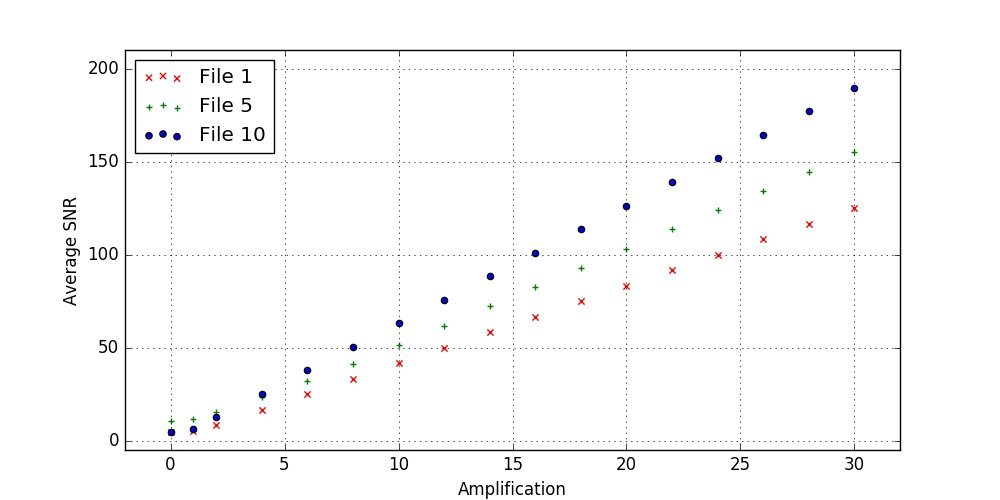
\includegraphics[scale = 0.4]{SNRs}
	\caption{A selected representative scatterplot\textemdash mean SNR plotted against the amplification of injected signal\textemdash generated by \texttt{matplotlib.pyplot}. The plots are the average maximum SNR values computed from each file at various amplifications of signals. There are three out of the ten series plotted. They represent the early, middle, and late stage of S6. One can see from Table \ref{tab:RMS} that File 1 contains the most noise, the noise in file 5 is among the middle, and file 10's noise is the second least. \label{fig:SNRs}}
\end{figure}
\par Consequently, the SNRs recovered from the unamplified injection (amplification equals one) are largely unreliable, which means there should be another method of calculating the SNRs\textemdash to use regression analysis to extrapolate the SNRs of the injected signal at the original amplitude in the background noise.
%---------------------------------------------------------------------------------------

\subsection{Computing the Linear Regression \label{sec:reg}}
Due to the nature of SNR, the amplification (signal power) should be positively correlated with the output. From Figure \ref{fig:SNRs} it can be seen that the y and x values are not only positively correlated, but they have a nice linear relationship. Therefore, linear regression \cite{linereg} was chosen as the model.
\par Before the computation of each linear regression, all of the data points at the first four amplifications were excluded, because they are not clean enough. In Figure \ref{fig:SNRs}, it can be seen that the first four points of each series cross and overlap each other. The reason for this ambiguity is probably the relatively high ratio of the strength of the background noise to that of the signal.
\par In general, the statistics in Table \ref{tab:extrapolation} make good sense. The fourth column of figures ($R^2$) indicate the fitness of my model: the closer the value is to one, the better the statistics fit the model \cite{r_squared}. That these values are so close to one means the model had been well chosen, and thus the extrapolations would be quite accurate. In addition, the intercepts are also very close to zero. Because SNR is the relative power of the signal over the background noise, it should theoretically be zero if there is no signal present. In reality, however, the SNR is never zero because of noise's partial matching with the template. Now that the intercepts are close to zero, the extrapolations have become more credible.
\begin{table}
	\caption{These are the statistics calculated from the mean-SNR series in section \ref{sec:SNR} by linear regression. The fifth column lists the extrapolations. \label{tab:extrapolation}}
	% Table generated by Excel2LaTeX from sheet 'Sheet1'
	\begin{tabular}{ccccc}
		\hline
		\hline
		File Number & Slope & Intercept & $R^2$ & Extrapolated Mean SNR \\
		\hline
		1 & 4.167  & -0.073  & 0.999999999511  & 4.094  \\
		2 & 4.371  & 0.093  & 0.999999985140  & 4.464  \\
		3 & 4.171  & -0.692  & 0.999999992354  & 3.479  \\
		4 & 5.151  & -0.487  & 0.999999995775  & 4.664  \\
		5 & 5.155  & 0.134  & 0.999959583093  & 5.290  \\
		6 & 6.164  & -0.042  & 0.999999998879  & 6.122  \\
		7 & 6.279  & 0.206  & 0.999999998734  & 6.485  \\
		8 & 5.953  & 0.178  & 0.999999998084  & 6.131  \\
		9 & 6.032  & -0.036  & 0.999999997650  & 5.996  \\
		10 & 6.328  & -0.201  & 0.999999999774  & 6.128  \\
		\hline
		\hline
	\end{tabular}
\end{table}
\par Finally, since the model of linear regression in this case is simply $SNR=Amplitude\times Slope + Intercept$, the mean SNR at amplification equals one were easily extrapolated, which gave the values in the fifth column in Table \ref{tab:extrapolation}. Therefore, the predicted maximum SNRs of GW150914 signal in the background noise of LIGO at various stages over S6 run were found. Overall, none of those SNRs would be significant enough to claim a detection. In the early stages where noises were high, the signal would be overwhelmed by the noise, while in the late stage where noises had been reduced, the maximum SNR would still not be significant enough. One can see from Figure \ref{fig:file1} that the SNR function of background noise is constantly around four with some spikes up to 6, regardless of that maximum around 3500 seconds due to hardware injection. Moreover, the SNR time functions in other nine files look very similar, mostly with SNR values of four, with a few spikes reaching up to six.
\begin{figure}
	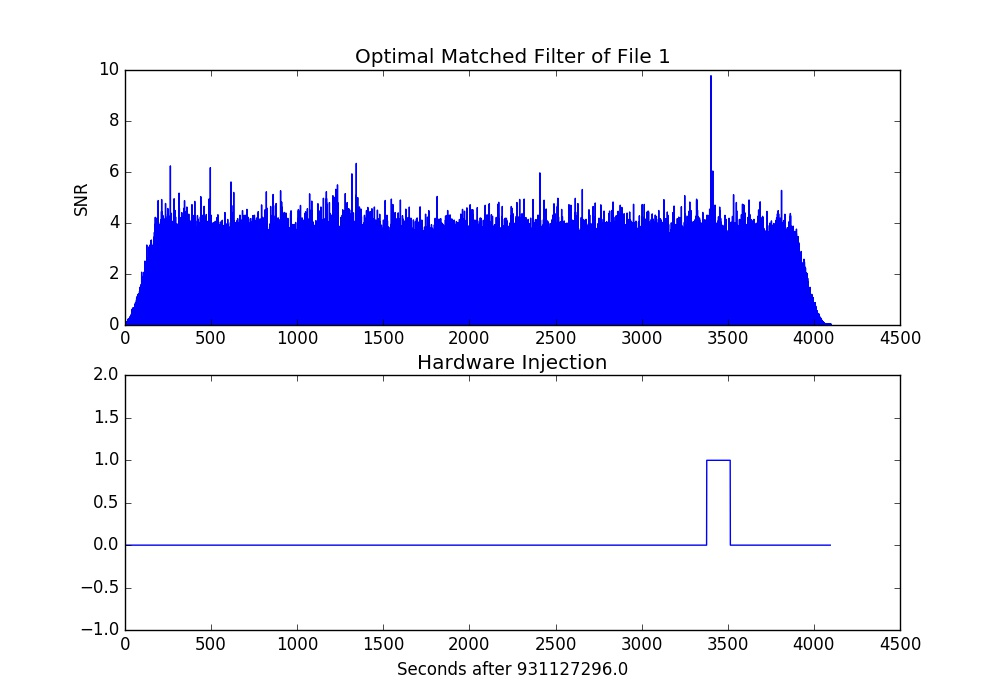
\includegraphics[scale = 0.35]{SNR}
	\caption{The upper image is the SNR function over the full span of file one. The lower image flags a hardware injection where there is a bulge in the graph. The highest spike in the upper graph is due to an injection indicated by the lower graph. \label{fig:file1}}
\end{figure}
%==========================================================


\section{Comparing S6 to Earlier Stages of LIGO \label{sec:compare}}
As the square root of power spectral density \cite{PSD}, amplitude spectral density (ASD) can serve as an indication of the amount of background noise as well. Figure \ref{fig:sensitivity2} suggests that the sensitivity of LIGO during S5 was not any better than that during S6, and Figure \ref{fig:sensitivity1} strongly suggests that the overall sensitivity of LIGO had been improved over time. As a result, it would be impossible for LIGO at stages prior to S6 to detect GW150914, for even the sensitivity at S6 was not high enough.
\begin{figure}
	\subfloat[Sensitivity of LIGO from S1 to S5 \label{fig:sensitivity1}]{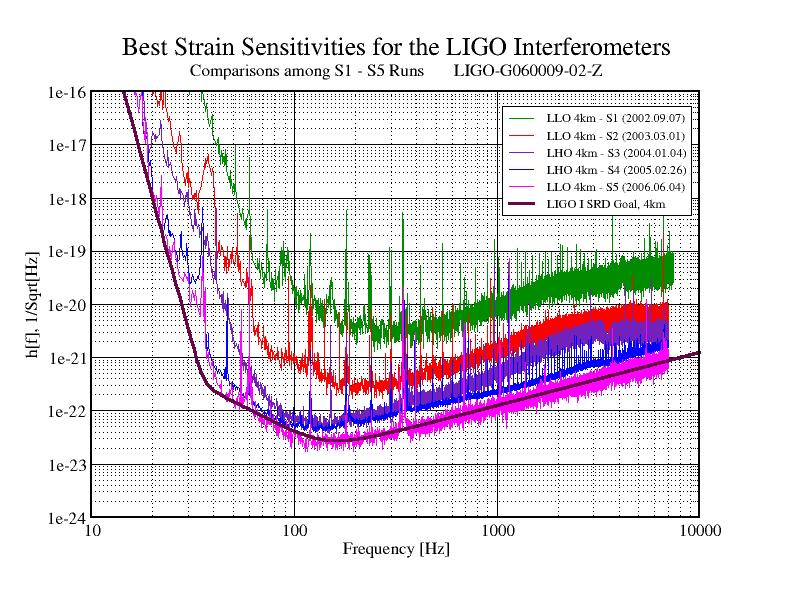
\includegraphics[width = 0.54\textwidth]{LIGOsensitivity}}
	\subfloat[Sensitivity of LIGO at S5 and S6 \label{fig:sensitivity2}]{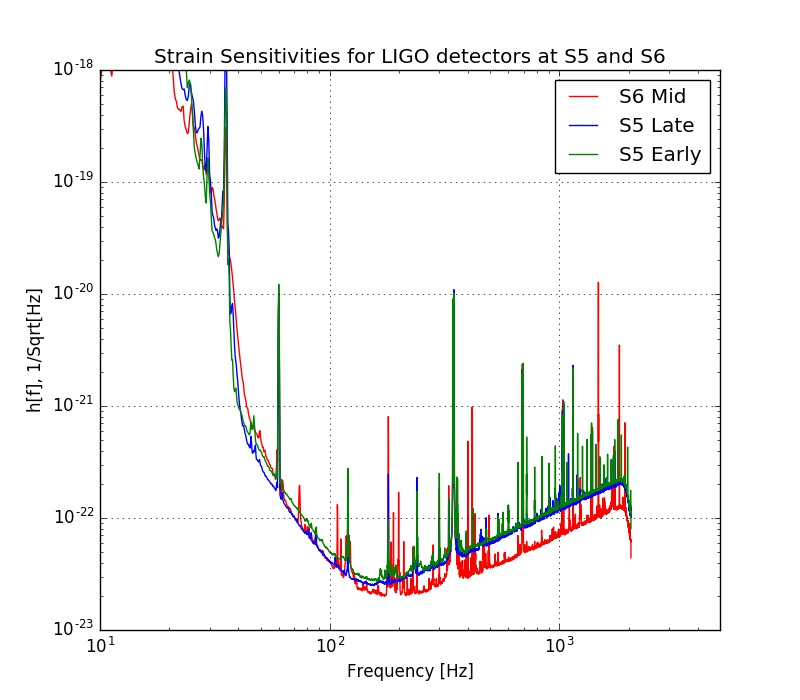
\includegraphics[width = 0.46\textwidth]{S5vsS6}}
	\caption{Left: a set of amplitude spectral density graphs of the backgound noise of LIGO during the five runs prior to S6. Source: \cite{nasa}. Right: the amplitude spectral density graphs of three strain data pieces during S5 and S6, computed by \texttt{matplotlib.mlab.psd()} and generated by \texttt{matplotlib.pyplot} The three files (S6 med, S5 late, and S5 early) are from the H1 detector and start at GPS time 947154944, 875126784, and 822124544.}
\end{figure}
%==========================================================


\section{Side Evidence}
 In fact, the subsequent successful detections of both a gravitational-wave event \cite{GW2} and a gravitational-wave candidate event \cite{Candidate,Observation1} also serve as evidence that the detection of GW150914 was not a coincidence. One can infer from these detections that the newest LIGO had finally become sensitive enough to make frequent detections. It appears that more detections will come in the near future.
%===============================================================
 
 
\section{Conclusion}
I found that the GW150914 event would not be loud enough to be detected by LIGO at S6 run. The signal could, at best, be identified as a candidate event at later stages where the sensitivity was relatively better, but its significance would be far from enough to claim a real detection. In short, LIGO in the S6 run was not sensitive enough to make this detection, not to mention the stages prior to S6 (e.g. S5), where the sensitivity was even worse. Besides, the other two subsequent detections have made it more likely that detecting GW150914 was just a beginning of a series of detections, triggered by the increased sensitivity. In conclusion, the detection of the GW150914 event was not a mere coincidence. In contrast, the successful detection was (and future detections will be) made possible by persistently upgrading the detectors.
%==========================================================


\section{Further Research}
Although the results indicate that earlier LIGO was not able to detect GW150914, it may become possible if the parameters that decide the strain amplitude of the gravitational waves were to change. As stated in section \ref{sec:GW}, the strain amplitude of gravitational waves measured at a certain point is inversely proportional to the distance from the source. Thus, if the distance from the binary system of GW150914 were to be halved, the amplitude of the signal would be doubled (or amplified by a factor of two). According to the regression model in section \ref{sec:reg}, the expected maximum SNR would be around ten, indicating a highly probable event. However, that would also mean the total number celestial bodies within the radius would be cut to roughly one eighth of the original number. Given the nonuniform distribution of stars and galaxies, the probability that a similar system exists within a shorter radius is hard to predict. Further investigation and presumably future detections will be needed to resolve this problem.
%===========================================================

\bibliography{Paper3,Paper1Background,Paper2Proposal}

%============================================================
\section{Appendix\textemdash Python Script \label{sec:Appendix}}
This is the main Python script used for my research. Please note that an automatic line break in this paper would cause an absence of line break operator \enquote{\textbackslash} or a line without the comment notation \enquote{\#} when one copies the script to a compiler.
\par First, the program completed the recovery on uninjected data. Then it superposed the unamplified data at five random points and did the same recovery. Then, instead of starting from raw data, it just superposed another signal with an amplification equal to the difference from the current one to the next one, and the program did the recovery for the next amplification. For example, if the program was now at an amplification of 10 and the next one was 12, it just superposed five signals amplified by a factor of two to the five according points.
\par This version is 2.7. In addition, the code was compiled and run by Anaconda2 (iPython). The total computational time was about 38 minutes.
	\lstset{
		basicstyle = \linespread{0.85} \ttfamily \scriptsize,
		breaklines = true,
		frame=single,
		language = python,
	}
\begin{lstlisting}
# Programmer: Tony Lu Zhehao
# From: 2AP2 International Cirriculum Center,
# Shenzhen Foreign Languages School, Shenzhen, China
# This script is to make and recover injections on LIGO's raw datafiles.
# It generally randomly pick 5 points in each datafile to work on.
# The recovery algorithm is adapted from the tutorial of GW150914 on LOSC.
# It has been very slightly altered, but 99% of it is the same.
# URL: https://losc.ligo.org/s/events/GW150914/LOSC_Event_tutorial_GW150914.html
# NOTICE:
# Highly recommend backing up the files, because the injections will not be
# easily removed.
# The output is the average SNR of each injection.

import h5py
import numpy as np
import matplotlib.pyplot as plt
import matplotlib.mlab as mlab
import scipy.signal as sig
import readligo as rl
from random import randint


#-- Sampling rate equals to 4096 Hz
fs = 4096

#-- Read in the waveform
temp_time, temp_strain = np.genfromtxt('GW150914_4_NR_waveform.txt').transpose()

#-- Read in the template
f_template = h5py.File('GW150914_4_template.hdf5', 'r')
template_p, template_c = f_template['template'].value
template = template_p + template_c * 1.j

# to remove effects at the beginning and end of the data stretch, window the data
# https://en.wikipedia.org/wiki/Window_function#Tukey_window
try:   dwindow2 = sig.tukey(template.size, alpha=1./8)  # Tukey window preferred, but requires recent scipy version 
except: dwindow2 = sig.blackman(template.size)          # Blackman window OK if Tukey is not available

# the length and sampling rate of the template MUST match that of the data.
datafreq = np.fft.fftfreq(template.size)*fs
df = np.abs(datafreq[1] - datafreq[0])
# prepare the template fft.
template_fft = np.fft.fft(template*dwindow2) / fs

# -- To calculate the PSD of the data, choose an overlap and a window (common to all detectors)
#   that minimizes \enquote{spectral leakage} https://en.wikipedia.org/wiki/Spectral_leakage
NFFT = 4*fs
psd_window = np.blackman(NFFT)
# and a 50% overlap:
NOVL = NFFT/2

#-- Set the amplifications of signal to be injected
A = [0,1,2] + range(4,31,2)

#-- Define the function to segment the segments into suitable segments
def slice_filter(dq, hw):
    #-- Cut the whole segment in to small ones of 60s, with spacing of 1s
    i = 0
    while i < len(dq):
        if dq[i].stop - dq[i].start < 32*fs:
            del dq[i]
            continue
        dq.insert(i, slice(dq[i].start, dq[i].start + 32*fs))
        dq[i+1] = slice(dq[i].stop + 1*fs, dq[i+1].stop)
        i += 1
    #-- Delete the segments with injection activated
    i = 0
    j = 0
    if len(hw) == 0:
        return dq
    while i < len(dq) and j < len(hw):
        #-- dq is 100% before hw
        if dq[i].stop < hw[j].start:
            i += 1
        #-- dq is 100% after hw
        elif dq[i].start > hw[j].stop:
            j += 1
        #-- dq and hw overlap
        else:
            del dq[i]

    return dq

#-- Prepare the files to work on
fileName = []
fileName.append('H-H1_LOSC_4_V1-931127296-4096')
fileName.append('H-H1_LOSC_4_V1-934846464-4096')
fileName.append('H-H1_LOSC_4_V1-941707264-4096')
fileName.append('H-H1_LOSC_4_V1-941785088-4096')
fileName.append('H-H1_LOSC_4_V1-947154944-4096')
fileName.append('H-H1_LOSC_4_V1-952623104-4096')
fileName.append('H-H1_LOSC_4_V1-959344640-4096')
fileName.append('H-H1_LOSC_4_V1-963629056-4096')
fileName.append('H-H1_LOSC_4_V1-967442432-4096')
fileName.append('H-H1_LOSC_4_V1-971407360-4096')


#===========================#
#========Main Part==========#
#===========================#
for name in fileName:

    #-- Prepare the document to record the table (SNR vs Ampli.)
    f = open(name + '.txt', 'w')

    #-- Load data from the original file
    rawFile = h5py.File(name + '.hdf5', 'r')
    strain_raw = rawFile['strain/Strain'].value
    CBCHIGH_CAT4 = (rawFile['quality/simple/DQmask'].value >> 4) & 1
    HW_CBC = (rawFile['quality/injections/Injmask'].value >> 0) & 1
    GPSstart = rawFile['meta/GPSstart'].value
    rawFile.close()

    #-- Load the file again which will be injected
    dataFile = h5py.File(name + '.hdf5', 'r+')
    strain = dataFile['strain/Strain']
    dqInj = dataFile['quality/injections/Injmask']

    #-- Getting the suitable segement lists
    segList = rl.dq_channel_to_seglist(CBCHIGH_CAT4)
    segList_HW = rl.dq_channel_to_seglist(HW_CBC)
    segList = slice_filter(segList, segList_HW)

    #-- Pick 10 (or if not more than 10, all) segments randomly
    inj_num = []
    if len(segList) <= 5:
        inj_num = range(0, len(segList))
        #-- If less than 5, throw a caution
        print 'Caution: there are less than five suitable spots in %s!' % name
        print '{0} only!'.format(len(segList))
    else:
        while len(inj_num) < 5:
            i = randint(0, len(segList)-1)
            if i in inj_num:
                continue
            inj_num.append(i)
    inj_num.sort()

    List = []
    for i in inj_num:
        List.append(segList[i])

    #-- Make and recover injections at each amplitude
    for k in range(0, len(A)):
        f.write('{0} '.format(A[k]))
        
        #-- Amplify the template with the difference to next amplification
        if k == 0:
            temp = temp_strain * (A[k])
        else:
            temp = temp_strain * (A[k] - A[k-1])

        #-- Make the injection to every piece
        SNRsum = 0
        
        for seg in List:
            #-- Injection starts at the middle
            inj_sample = seg.start + 16*fs
            #-- Superpose the waveform to the signal
            for j in range(0, temp.size):
                strain[inj_sample + j] += temp[j]
                    
            #-- Injection Recovery --#
            #using the segments in the above section
            data = strain[seg]

            # to remove effects at the beginning and end of the data stretch, window the data
            # https://en.wikipedia.org/wiki/Window_function#Tukey_window
            try:   dwindow = sig.tukey(data.size, alpha=1./8)  # Tukey window preferred, but requires recent scipy version 
            except: dwindow = sig.blackman(data.size)          # Blackman window OK if Tukey is not available

            #-- Calculate the PSD of the data.  Also use an overlap, and window:
            # This is where the only change is made, I replaced the PSD of the 32-s segment with
            # that of the whole file, because when the file is small the PSD will be greatly affected by the
            # signal in the file, whereas we only want the PSD of the background noise. So taking the PSD
            # of a much larger interval can help eliminating the effect.
            data_psd, freqs = mlab.psd(strain_raw, Fs = fs, NFFT = NFFT, window=psd_window, noverlap=NOVL)

            # Take the Fourier Transform (FFT) of the data and the template (with dwindow)
            data_fft = np.fft.fft(data*dwindow) / fs

            #-- Interpolate to get the PSD values at the needed frequencies
            power_vec = np.interp(np.abs(datafreq), freqs, data_psd)

            #-- Calculate the matched filter output in the time domain:
            # Multiply the Fourier Space template and data, and divide by the noise power in each frequency bin.
            # Taking the Inverse Fourier Transform (IFFT) of the filter output puts it back in the time domain,
            # so the result will be plotted as a function of time off-set between the template and the data:
            optimal = data_fft * template_fft.conjugate() / power_vec
            optimal_time = 2*np.fft.ifft(optimal)*fs

            #-- Normalize the matched filter output:
            # Normalize the matched filter output so that we expect a value of 1 at times of just noise.
            # Then, the peak of the matched filter output will tell us the signal-to-noise ratio (SNR) of the signal.
            sigmasq = 1*(template_fft * template_fft.conjugate() / power_vec).sum() * df
            sigma = np.sqrt(np.abs(sigmasq))
            SNR_complex = optimal_time/sigma

            # shift the SNR vector by the template length so that the peak is at the END of the template
            peaksample = int(data.size / 2)  # location of peak in the template
            SNR_complex = np.roll(SNR_complex,peaksample)
            SNR = abs(SNR_complex)

            #-- Find the time and SNR value at maximum:
            indmax = np.argmax(SNR)
            SNRmax = SNR[indmax]
            SNRsum += SNRmax

        SNR_avr = SNRsum / len(inj_num)
        f.write('{0}\n'.format(SNR_avr))
        dataFile.flush()

        print '%s at amplification = {0} finished.'.format(A[k]) % name

    dataFile.close()
    f.close()
\end{lstlisting}
%==========================================================

\end{document}
%EOF